\documentclass[a4paper,12pt]{article}
\usepackage[english,polish]{babel}
\usepackage{polski}
\usepackage[utf8]{inputenc}
\usepackage{graphicx}
\usepackage{array}
\newcommand{\HRule}{\rule{\linewidth}{0.5mm}}

\setlength\fboxsep{1pt}
\setlength\fboxrule{0pt}
\def \tscale {0.3}

\begin{document}
\begin{titlepage}
	\begin{center}
		
\includegraphics[width=0.4\textwidth]{data/logo.jpg} \\[1cm]
		\textsc{\LARGE Technika Mikroprocesorowa} \\[0.8cm]
		\HRule \\[0.4cm]
		{ \huge \bfseries Gesture Processing Library - Projekt} \\[0.4cm] 
%touch to dotyk;)
%racja
		\HRule \\[1.5cm]
	\end{center}
	\begin{minipage}{0.4\textwidth}
		\begin{flushleft} \large
		\emph{Autorzy:} \\
		Michał \textsc{Janiec} \\
		Bartosz \textsc{Polnik}
		\end{flushleft}
	\end{minipage}
\end{titlepage}
\thispagestyle{empty}



\section{\Large Temat} \ \\[0.1cm]
\indent Stworzenie niskopoziomowej biblioteki do przetwarzania gestów, dedykowanej dla mikroprocesorów jedno-układowych.

\section{\Large Cel} \ \\[0.1cm]
\indent Celem projektu jest przede wszystkim stworzenie ww. biblioteki pozwalającej na wygodne korzystanie z technologi multi-touch na różnorodnych urządzeniach. Ponadto utworzona zostanie aplikacja na platformę Android służąca zaprezentowaniu działania biblioteki. Jej zadaniem będzie odczytywanie gestów wykonanych przez użytkownika i wyświetlanie ich nazw.

\section{\Large Opis zagadnienia} \ \\[0.1cm]
\indent Zadaniem biblioteki będzie odczytywanie gestów z urządzenia dotykowego. Biblioteka będzie periodycznie odczytywać stan urządzenia (wejście biblioteki). Na tej podstawie będzie rozpoznawać ruchy, które będzie dopasowywać do listy gestów. Po rozpoznaniu gest informacja o wykonanym geście zostanie umieszczona w kolejce gestów (wyjście biblioteki). Użytkownik biblioteki powinien periodycznie sprawdzać czy coś pojawiło się w kolejce i samodzielnie przetwarzać jej zawartość. Gesty będą dodawane do biblioteki w czasie kompilacji. Biblioteka zostanie napisana w języku C bez użycia zewnętrznych bibliotek.



\section{\Large Lista gestów} \ \\[0.1cm]
\indent W celu uniknięcia niejednoznaczności proponujemy anglojęzyczne nazwy gestów.\\

\begin{tabular}{|>{\bf}p{2cm}|c|p{4cm}|p{5cm}|}
\hline	\textbf{Nazwa}&\textbf{Rysunek}&\textbf{Opis}&\textbf{Parametry}\\ \hline 
	
     Tap & \fbox{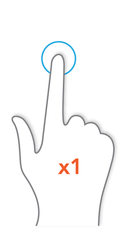
\includegraphics[scale=\tscale]{data/Tap.png}} & 
		Pojedyncze stuknięcie w multi-touch. & 	Pozycja (x,y)  \\ \hline
		
	 Double Tap & \fbox{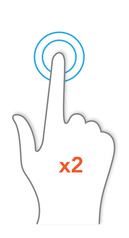
\includegraphics[scale=\tscale]{data/Double_Tap.png}} & 
	 	Szybkie podwójne stuknięcie w multi-touch. & Pozycja (x,y)  \\ \hline
	 	
	 Press & \fbox{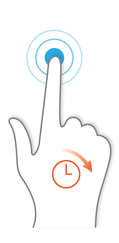
\includegraphics[scale=\tscale]{data/Press.png}} &
	 	Stuknięcie i przytrzymanie palca przez dłuższy czas. & 	Pozycja(x,y) \\ \hline
	 	
	 Move & \fbox{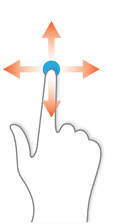
\includegraphics[scale=\tscale]{data/Move}} &
	 	Przesunięcie palca w dowolnym kierunku. & Up/Down/Left/Right, Pozycja(x,y) \\ \hline
	 	
	 Rotate & \fbox{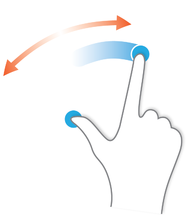
\includegraphics[scale=\tscale]{data/Rotate}} &
	 	Obrót w lewo lub w prawo. & Left/Right Obrót, (kąt) \\ \hline
	 
	 Flick & \fbox{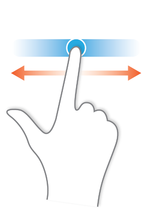
\includegraphics[scale=\tscale]{data/Flick}} &
	 	Przesunięcie palca w lewo lub prawo i puszczenie. &	Left/Right, Pozycja(x,y) \\ \hline
	 	
\end{tabular}

\begin{tabular}{|>{\bf}p{2cm}|c|p{4cm}|p{5cm}|}
\hline	\textbf{Nazwa}&\textbf{Rysunek}&\textbf{Opis}&\textbf{Parametry}\\ \hline 

	 Scroll & \fbox{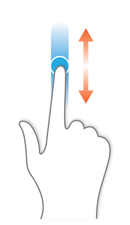
\includegraphics[scale=\tscale]{data/Scroll}} &
	 	Przesunięcie palca w górę lub w dół i puszczenie. &	Up/Down, Pozycja(x,y) \\ \hline
	 
	 Zoom & \fbox{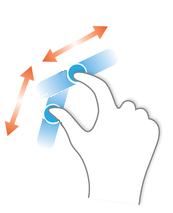
\includegraphics[scale=\tscale]{data/Zoom}} &
	 	Przybliżenie lub oddalenie palca wskazującego i kciuka do siebie. &	In/Out, Przybliżenie (liczba) \\ \hline
	 
	 Two Finger Scroll & \fbox{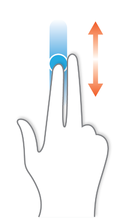
\includegraphics[scale=\tscale]{data/TwoFingerScroll}} &
	 	Przesunięcie dwóch palców równolegle w górę lub w dół. & Up/Down, Pozycja(x,y) \\ \hline
		
\end{tabular}

\section{\Large Lista wymagań dla biblioteki}
	\subsection*{a) Wymagania Niefunkcjonalne}
	\begin{itemize}
		\item Platforma docelowa - Dowolny mikroprocesor jedno-układowy.
		\item Oszczędność pamięci.
		\item Nie korzystanie z koprocesora.
		\item Optymalność algorytmiczna.
	\end{itemize}
   		
	\subsection*{b) Wymagania Funkcjonalne}
	\begin{itemize}
		\item Rozpoznawanie gestów z powyższej listy.
		\item Wystawianie eventów (zdarzeń).
	\end{itemize}

\section{\Large Aplikacja testowa}
Celem aplikacji będzie wizualne zaprezentowanie możliwości i cech biblioteki. Na ekranie wydzielony będzie obszar, w obrębie którego użytkownik będzie wykonywał ruch, a w odpowiedzi dostawał będzie informację o najbliższym dopasowaniu do predefiniowanego gestu zwróconego przez bibliotekę.

\section{\Large Lista wymagań dla aplikacji testowej}
	\subsection*{a) Wymagania Niefunkcjonalne}
	\begin{itemize}
		\item Platforma docelowa - Android.
		\item Użycie biblioteki stworzonej podczas realizacji projektu.
		\item Prosty interfejs użytkownika.
	\end{itemize}
   		
	\subsection*{b) Wymagania Funkcjonalne}
	\begin{itemize}
		\item Możliwość przetestowania wielu gestów wspieranych przez bibliotekę.
		\item Prezentacja dokładnych informacji o rozpoznanym geście.
	\end{itemize}

	
\section{\Large Wstępny Harmonogram}
\begin{tabular}{l p{10cm}}
	\textsc{Data} & \textsc{Podsumowanie} \\[0.1cm]
	 29.10.2012   &  Określenie harmonogramu prac oraz zakresu projektu\\[0.1cm]
	 19.11.2012   &  Wstępny prototyp umożliwiający wczytanie oraz przetworzenie jednego gestu\\[0.1cm]
	 03.12.2012   &  Wstępny prototyp umożliwiający wczytanie oraz przetworzenie wielu gestów\\[0.1cm] 
	 17.12.2012   &  Działająca wersja aplikacji umożliwiająca wczytanie, przetworzenie oraz interpretację gestów w formie widzialnej dla użytkownika\\[0.1cm]
	 07.01.2013   &  Oddanie działającej biblioteki
\end{tabular}
\end{document}